\chapter{Propuesta de solución}\label{chapter:Solution}

La implementación del sistema está dividida en cuatro módulos: Núcleo, trabajo con vecindades, evaluación de soluciones y generador de funciones de exploración.

\begin{itemize}
	\item Núcleo (\textbf{Core}): En este módulo se implementan las clases a partir de las cuales se pueden describir las soluciones y criterios de vecindad para Problemas de Enrutamiento de Vehículos.
	\item Trabajo con vecindades (\textbf{Neigh}): Se implementa el Árbol de Vecindad a partir del cual se genera soluciones con distintas formas de exploración de vecindades.
	\item Evaluación de soluciones (\textbf{Eval}): Se implementa el grafo de evaluación con el que se obtiene el costo de soluciones vecinas a partir de cómo se evalúa una solución.
	\item Generador de funciones de exploración (\textbf{Generator}): Este módulo contiene el código que permite generar funciones de exploración para combinar estrategias de exploración y selección.
\end{itemize}

Estos cuatro módulos ya existían antes de que se desarrollara el presente trabajo. En las secciones siguientes se describen los detalles de cada uno de estos módulos, cómo se combinaron y qué modificaciones se le hizo a cada uno para implementar esta tesis. En ela sección \ref{2-core} se describe el módulo \textbf{core}. En la sección \ref{2-neigh} se describe el módulo \textbf{neigh}. En la sección \ref{2-eval} se describe el módulo \textbf{eval}. Por último, en la sección \ref{2-generator} se describe el módulo \textbf{generator}

\section{Vrp-Core}\label{2-core}

En el módulo \textit{core} se definen funciones para inicializar el sistema, así como implementaciones de algoritmos de búsqueda local que utilizan funciones del sistema para explorar vecindades.

También se define un conjunto de clases que permiten describir soluciones para un Problema de Enrutamiento de Vehículos. A partir de esas soluciones se construye el grafo de evaluación.

También se definen clases que permiten definir los datos necesarios para resolver problemas específicos. Por ejemplo, para CVRP es necesaria la demanda de cada cliente y la matriz que guarda la distancia entre cada par de clientes. Para el Problema con backhaul, se define también una lista que guarda los tipos de cada cliente. En el capítulo \ref{chapter:Tutorial} se discute cómo ampliar el sistema para definir otras variantes de VRP.

Además, en este módulo se tiene clases que representan las operaciones que conforman los criterios de vecindad (como seleccionar ruta o insertar cliente).

Para el desarrollo de esta tesis, no se añadió código al módulo \textit{core}. Por el contrario, se desecharon secciones de código que quedaron obsoletas. Por ejemplo, en la versión anterior se utilizaba algo llamado \textit{solución de trabajo}, que era copia de la solución actual sobre la que se realizaban las modificaciones para evaluar vecinos eficientemente. Como esta tesis las evaluaciones se hacen mediante el Grafo de Evaluación, las \textit{soluciones de trabajo} quedan obsoletas. En la versión anterior se tenía también unos mecanismos con los que se exploraba vecindades, que al incorporar el Árbol de vecindad fueron desechados.

Una vez definidas las clases que permiten crear una solución, definir características de un problema, y definir un problema, es posible construir un Árbol de Vecindad. Esto se hace en el módulo \textbf{neigh}.

\section{Vrp-neigh}\label{2-neigh}
En este módulo se define el Árbol de Vecindad como una clase que se construye a partir de un problema, una solución y un criterio de vecindad. 

El Árbol de Vecindad permite crear iteradores (o generadores) de soluciones. La función que se usa para crear el iterador depende del tipo de exploración que se desee (como \textbf{exhaustive-exploration} o \textbf{random-exploration}). Cada vez que se ejecuta un iterador, se obtiene la lista de operaciones que se aplican a la solución actual para generar un vecino, o \textbf{nil} en caso de que se no queden vecinos por analizar. Esta condición varía según el tipo de exploración. Por ejemplo, para la exploración exhaustiva se generan todas las soluciones de la vecindad, mientras que en una aleatoria se genera una cantidad predefinida de vecinos. 

En el trabajo original donde se desarrolló este módulo, las clases se definían de manera distinta a como se definen en el módulo \textbf{core}. Por tanto, en el presente trabajo se cambió las definiciones de clases para, en todos los casos, utilizar \textbf{def-vrp-class}. De esta forma, todas las clases de \textbf{neigh} se volvieron consistentes con el resto del sistema. También se agregó la función \textbf{random-exploration} para obtener el iterador de exploración aleatoria.

A partir del Árbol de Vecindad se obtienen iteradores que generan vecinos en forma de lista de operaciones de vecindad. Al aplicar estas operaciones sobre la solución actual se forma una solución cuyo costo se puede calcular utilizando el Grafo de Evaluación.

\section{Vrp-eval}\label{2-eval}
En esta sección se implementa el Grafo de Evaluación, que como se explicó en la sección \ref{2-eval}, tiene tres tipos de nodos: Nodos que representan los elementos de la solución (clientes, depósitos), nodos acumuladores (como el costo total), y nodos operacionales (aumentar valor, disminuir valor). 

El grafo contiene los siguientes elementos:

\begin{itemize}
	\item Una copia de la solución actual.
	\item Una lista con los nodos del grafo.
	\item Una correspondencia entre cada elemento de la solución y el nodo del grafo que lo representa.
	\item Una correspondencia entre los nodos acumuladores y las variables a las que representan.
	\item El valor del costo total de la solución.
\end{itemize}

Para incorporar este módulo al sistema hubo que reimplementarlo prácticamente desde cero. En su versión anterior, el código del grafo de evaluación estaba aislado del módulo \textbf{core} y, por tanto, este grafo no se podía construir a partir de las clases para describir soluciones que utiliza el sistema. Con el desarrollo de este trabajo se crearon métodos y clases de inicialización, construcción y modificación de grafo compatibles con las clases de \textbf{core}.

Para inicializar un grafo sólo es necesaria la solución actual. La inicialización consiste en convertir los elementos de la solución (clientes, depósitos, vehículos) en los nodos que los representan.

Para terminar de construir el grafo, se debe definir y ejecutar el código de evaluación de la solución inicial a partir de funciones definidas en el sistema. Algunos ejemplos de estas funciones son:

\begin{itemize}
	\item \textbf{def-var}: Recibe un nombre y un valor inicial. Inicializa un nuevo nodo acumulador y se lo hace corresponder con el nombre recibido.	
	\item \textbf{increment-distance}: Recibe dos clientes, una variable asociada a un nodo acumulador y la matriz de distancia. Crea y evalúa un nodo operacional que incrementa el valor almacenado en el nodo correspondiente a la variable en una cantidad igual a la distancia entre los clientes.
	\item \textbf{decrement-demand}: Recibe un cliente y una variable asociada a un nodo acumulador. Crea y evalúa un nodo operacional que recibe el cliente y decrementa el valor del nodo correspondiente a la variable en una cantidad igual a la demanda del cliente.
	\item \textbf{increment-value}: recibe dos variables. Incrementa el valor del nodo asociado a la segunda variable en una cantidad igual al valor del nodo asociado a la primera variable.
	\item \textbf{apply-penalty}: Recibe dos variables y un factor de penalización. Crea y evalúa un nodo operacional que recibe el nodo asociado a la primera variable y, en caso de que este tenga valor negativo, aumenta el valor del nodo asociado a la segunda variable en una cantida que depende del factor de penalización.
	\item \textbf{return-value}: Recibe una variable y marca su nodo asociado como el nodo que contiene el costo total de la solución. A partir del punto en que se invoca, la propiedad \textit{output} (salida o costo total) del grafo referencia a este nodo.
\end{itemize}

Todas las funciones de construcción de grafo reciben también como parámetro la instancia del grafo sobre el que se está trabajando. En el capítulo \ref{chapter:Tutorial} se discutirá la ampliación del sistema con nuevos métodos. 

A continuación se muestra el pseudo-código que evalúa una solución de CVRP.

\begin{lstlisting}
def-var total-distance (initial-value = 0)
loop for r in solution-routes do
	def-var route-distance (initial-value = 0)
	def-var route-capacity (initial-value = vehicles-capacity)	
	loop for c in r-clients do
		increment route-distance in distance between r-previous-client c 
		decrement route-demand in client-capacity	
	set r-previous as c
	increment total-distance in route-distance
	apply-penalty in total-distance with route-capacity
return-value total-distance

\end{lstlisting}

En las líneas 1 se usa def-var para inicializar, y asociar a su respectivo nodos, la variable que almacenan el costo total de la solución. Luego se analizan las rutas de la solución. Por cada ruta se definen, y asocian a sus respectivos nodos, variables que almacena el costo (línea 3) y la capacidad restante de la ruta (líneas 4). A continuación se analizan los clientes de la ruta actual. Se incrementa el valor del nodo asociado al costo de la ruta en una cantidad igual a la distancia del cliente actual y el cliente previo (el cliente previo inicial de la ruta es el depósito)(línea 6). También se decrementa el valor del nodo asociado a la capacidad de la ruta en una cantidad igual a la demanda del cliente actual (línea 7) Una vez se analiza una ruta, se aumenta el valor del nodo asociado al costo total de la solución en una cantidad igual al costo de esta ruta (línea 8) y se penaliza el nodo de costo total en caso de ser necesario (línea 9). Finalmente se declara como nodo salida al nodo asociado a la variable de distancia total (línea 10).

En su versión anterior, el módulo \textbf{eval} tampoco era compatible con las clases de \textbf{core} que describen operaciones de vecindad. Para aplicar y deshacer en el grafo las operaciones de vecindad que utiliza el sistema se implementaron las funciones \textbf{do-core-operations} y \textbf{undo-core-operations}.

\textbf{Do-core-operations} recibe una lista de operaciones y el grafo sobre el cual estas se ejecutan. Las operaciones se hacen en orden. Los nodos que representan elementos de la solución se insertan o eliminan del grafo y los nodos operacionales que dependan de ellos se ejecutan o deshacen. Por ejemplo, dado el grafo representado en la figura \ref{fig:eval-graph-2}, al ejecutar el siguiente código:

\begin{figure}
	\centering
	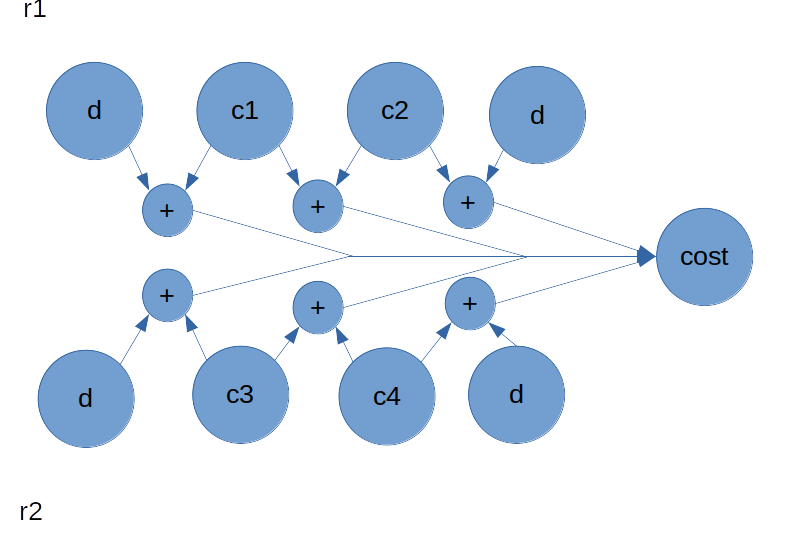
\includegraphics[width=0.9\linewidth]{Graphics/eval-graph-2}
	\caption{Grafo de evaluación que representa la solución $s1$ de VRP clásico.}
	\label{fig:eval-graph-2}
\end{figure}

\begin{lstlisting}
do-core-operations (graph ((op-select-client 1 from route 1)
										(op-insert-client 1 to route 3 in 2))
\end{lstlisting}

Se obtiene el grafo representado en \ref{fig:eval-graph-4}. En este punto, la propiedad \textit{output} del grafo (Que en este caso hace referencia al nodo \textit{cost}) tiene el costo total de la nueva solución.

Para deshacer operaciones que se hicieron previamente en un grafo se ejecuta la función \textbf{undo-core-operations}. Por ejemplo, al ejecutar el siguiente código sobre el grafo representado en la figura \ref{fig:eval-graph-4}:

\begin{figure}
	\centering
	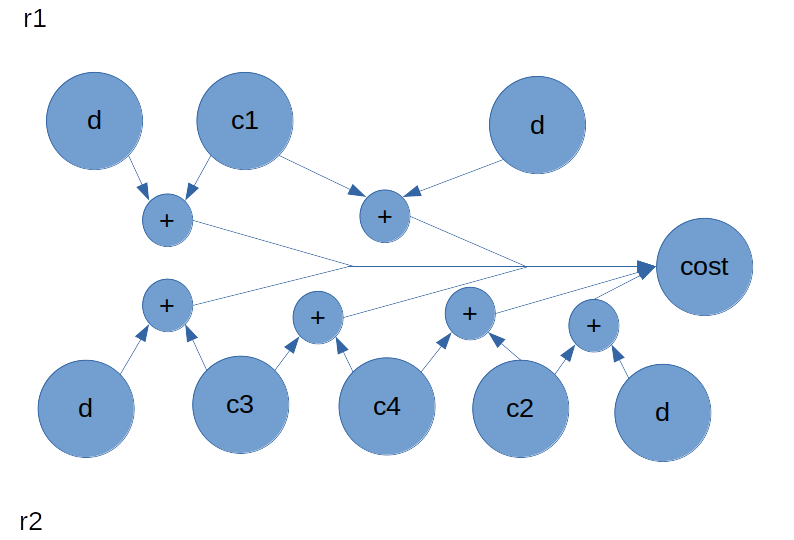
\includegraphics[width=0.9\linewidth]{Graphics/eval-graph-4}
	\caption{Grafo de evaluación que representa la solución $s1$ de VRP clásico luego de aplicada una instancia de $rarb$}
	\label{fig:eval-graph-4}
\end{figure}

\begin{lstlisting}
undo-core-operations (graph ((op-select-client 1 from route 1)
											(op-insert-client 1 in route 3 in 2))
\end{lstlisting}

Se obtiene nuevamente el grafo representado por \ref{fig:eval-graph-2} y el valor almacenado en \textit{cost} vuelve a ser el costo total de la solución original.

Una vez que se definen funciones que generan y evalúan soluciones, sólo resta utilizarlas en exploraciones de vecindades. De eso se habla en la siguiente sección.

\section{Vrp-generator}\label{2-blueprint}
Una vecindad se puede analizar con distintas estrategias de exploración y selección. Cada vez que se combina una estrategia de exploración con una de selección se obtiene una manera diferente de analizar la vecindad. A cada una de estas combinaciones, en este trabajo se les llama función exploradora de la vecindad. Programar estas funciones exploradoras es un proceso con alto consumo de tiempo de trabajo humano. En \cite{Heidy} se propone un mecanismo para automatizar la creación de funciones exploradoras a partir de cualesquiera estrategias de exploración y selección, con un esfuerzo mínimo. Esto significa que ya no es necesario programar todas las funciones de exploración diferentes, lo cual agiliza el tiempo de desarrollo. Para esto, se utilizan las ventajas del Sistema de Objetos de Common Lisp (CLOS), en particular las combinaciones de métodos y la facilidad que brinda el lenguaje para generar código fuente en tiempo de ejecución.

Las posibles estrategias de exploración y selección se representan como clases y los criterios de vecindad mediante una lista de operaciones. En \cite{Heidy} se tiene una un mecanismo que recibe una estrategia de exploración, una de selección y un criterio, y devuelve una función que dada una solución explora la vecindad correspondiente a esas entradas.

La versión del módulo \textbf{generator} que se hizo en \cite{Heidy} utilizaba en las funciones de exploración que se generaban, elementos de \textbf{core} que con este trabajo quedaron obsoletos. Por tanto, parte de los mecanismos desarrollados en \cite{Heidy} también quedaron obsoletos.

En la versión anterior las vecindades se exploraban con cadenas de ciclos que mezclaban las operaciones. En el presente trabajo, esto se hace con un único ciclo que genera soluciones a partir del iterador del Árbol de Vecindad. Por otro lado, los vecinos se evaluaban mediante \textit{soluciones de trabajo} y esto ahora se hace a mediante el Grafo de Evaluación.

En este trabajo se define un nuevo generador de funciones que utiliza un Árbol de Vecindad y que, además, en lugar de ceribir una solución, ahora reciven un Grafo de Evaluación.

En \cite{Heidy} el código de una función de exploración (y por tanto, el código que se genera a partir de la función generadora) está dividido en 5 regiones comunes para cualquier exploración:

\begin{itemize}
	\item Inicializaciones de variables.
	\item Ciclos que definen cómo realizar la exploración (dependen del criterio).
	\item Instrucciones que se ejecutan dentro de los ciclos.
	\item Instrucciones que se ejecutan fuera de los ciclos.
	\item Valores que se retornan.
\end{itemize}

El siguiente pseudo-código muestra un ejemplo de función exploradora para el criterio \textit{mover cliente en cualquier posición de posición dentro de su ruta} con estrategia de exploración exhaustiva y con selección de mejor vecino. Esta función recibe una solución (\textbf{solution}) como argumento.

\begin{lstlisting}
set wc as working-copy of solution
set ops-list as nil
set current-cost as 0
set best-cost as 0
set best-neighbor as nil
set result-solution as nil

loop foreach route r:
	loop foreach client c:
		loop foreach pos p:
			
			set current-ops-list as (select-route-r,
												 select-client-c,
												 insert-client-c-in-route-r-in-position-p)
			set current-cost as apply-operations(wc current-ops-list)
			if (current-cost < best-cost) then:
				set best-neighbor as current-ops-list
				set best-cost as current-cost
				
if (best-neighbor exists) then
	set result-solution as operations best-neighbor applied over solution
	
return result-solution


\end{lstlisting}

En las líneas 1-6 seinicializan las variables variables necesarias. En las líneas 8-10 se crean los ciclos que definen cómo realizar la exploración, por cada operación del criterio se hace un ciclo. Las líneas 12-18 contienen el código dentro de los ciclos, se obtiene el costo actual a partir de la \textit{solución de trabajo} y en caso de ser menor que el actual mejor costo, se actualiza \textbf{best-cost} y \textit{best-neighbor}. Las líneas 20-21 tienen el código fuera de los ciclos, en caso de haberse encontrado un mejor vecino, se aplican sus operaciones sobre la solución actual para obtener la nueva solución. La línea 23 retorna la solución encontrada.

En este trabajo, la sección de los ciclos que definen cómo realizar la exploración se cambia por un único ciclo cuya condicional depende de la estrategia. El sigiente pseudo-código muestra la implementación del ejemplo anterior generado por el sistema desarrollado en esta tesis. Esta función recibe un grafo (\textbf{graph}) como parámetro.

\begin{lstlisting}
set neigh-tree as build-neigh-tree with criteria and graph-solution
set generator as exhaustive-exploration(neigh-tree)
current-ops-list as funcall(generator)

set best-cost as 0
set best-neighbor as nil

cicle while (current-ops-list exists)
			
			do-core-operations (current-solution graph)
			set current-cost as output of graph
			undo-core-operations (current-solution graph)
			if (current-cost < best-cost) then:
				set best-neighbor as current-ops-list
				set best-cost as current-cost
			set current-ops-list as funcall(generator)

if (best-neighbor exists) then
	do-core-operations best-neighbor over graph

return graph-current-solution
\end{lstlisting}

En la línea 8 se sustituye el código de la región de los ciclos por un único ciclo que se ejecutará mientras se cumpla su condición (en este caso, que el generador retorne un vecino). Además, la función ahora genera los vecinos a partir de un Árbol de Vecindad y en lugar de recibir una solución como argumento, recibe el grafo asociado a esa solución mediante el cual se obtiene el costo de los vecinos.

En este capítulo se exlicaron las características de cada módulo de este trabajo. El siguiente capítulo explica paso a paso cómo utilizar el sistema para resolver variantes de VRP. 










